\subsection{Архитектура средства обнаружения аномалий}

Разрабатываемое программное средство должно быть ориентировано на работу в условиях распределённой инфраструктуры и учитывать особенности функционирования Kubernetes-кластера, в частности высокую динамичность среды, большое количество генерируемых событий и необходимость обработки потоковых данных в режиме, близком к реальному времени.

В качестве источника данных используются audit-логи Kubernetes, агрегируемые и хранящиеся в системе OpenSearch. Для выполнения анализа данные извлекаются из хранилища, проходят этап предобработки и преобразуются в формат, пригодный для подачи на вход НС. Ключевым элементом системы является модель обнаружения аномалий на основе AE, позволяющая выявлять отклонения на основе ошибки реконструкции последовательностей. Такой подход обеспечивает возможность обнаружения ранее неизвестных типов аномалий без необходимости наличия размеченных данных.

Архитектура разработанного программного средства построена по принципу \textit{Master--Worker} и ориентирована на разделение управляющих и вычислительных функций между отдельными компонентами системы. Такой подход позволяет обеспечить асинхронную обработку задач, упростить масштабирование вычислительной части и повысить устойчивость системы к росту объёма анализируемых данных.

Общая схема архитектуры программного средства представлена на рисунке~\ref{fig:system_architecture}. В состав системы входят центральный компонент \textit{Master}, реализующий интерфейс для взаимодействия с пользователем, а также набор вычислительных узлов \textit{Worker}, выполняющих обучение нейросетевых моделей и детектирование аномалий. Взаимодействие между компонентами осуществляется посредством очереди задач, реализованной с использованием брокера сообщений \textit{Redis}, что позволяет отделить пользовательские операции от ресурсоёмких вычислений.

\begin{figure}
    \centering
    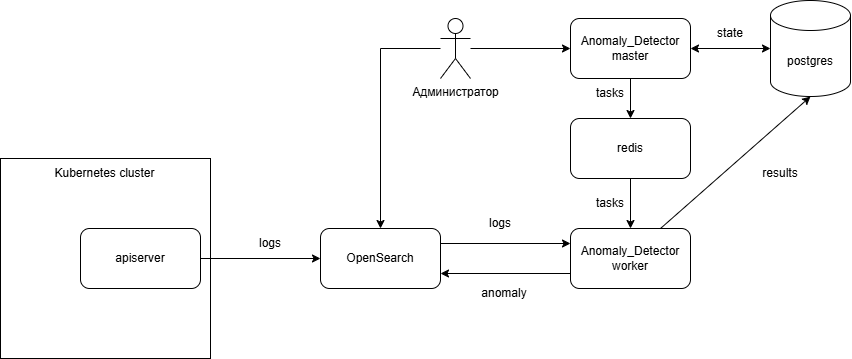
\includegraphics[scale=0.5]{inc/images/system_architecture}
    \caption{Архитектура программного средства обнаружения аномалий}
    \label{fig:system_architecture}
\end{figure}

Компонент \textit{Master} выполняет функции управления системой. Через него осуществляется аутентификация пользователей, создание и настройка интеграций с источниками данных, управление объектами моделей, а также запуск задач обучения и детектирования. Кроме того, \textit{Master} отвечает за хранение и обработку метаданных, связанных с пользователями, моделями, задачами и результатами выполнения.

Компонент \textit{Worker} предназначен для выполнения вычислительно затратных операций. В частности, он обеспечивает извлечение audit-логов из OpenSearch, преобразование данных с помощью конвейера формирования признаков, формирование обучающих последовательностей, обучение модели НС и последующее выявление аномальных событий.

Компонент \textit{Redis} выполняет функции брокера сообщений между \textit{Master} и \textit{Worker}-узлами.

В качестве хранилища метаданных используется \textit{PostgreSQL}. В базе данных фиксируются сведения о пользователях, интеграциях, моделях, задачах, результатах обработки и метриках обучения. Использование реляционной СУБД позволяет поддерживать целостность данных и удобно реализовать связи между сущностями системы.

Источником исходных данных для анализа выступает OpenSearch, в котором хранятся audit-логи Kubernetes-кластера.

Структура базы данных отражает основные сущности предметной области и их взаимосвязи. Диаграмма базы данных представлена на рисунке~\ref{fig:db_uml}.

\begin{figure}
    \centering
    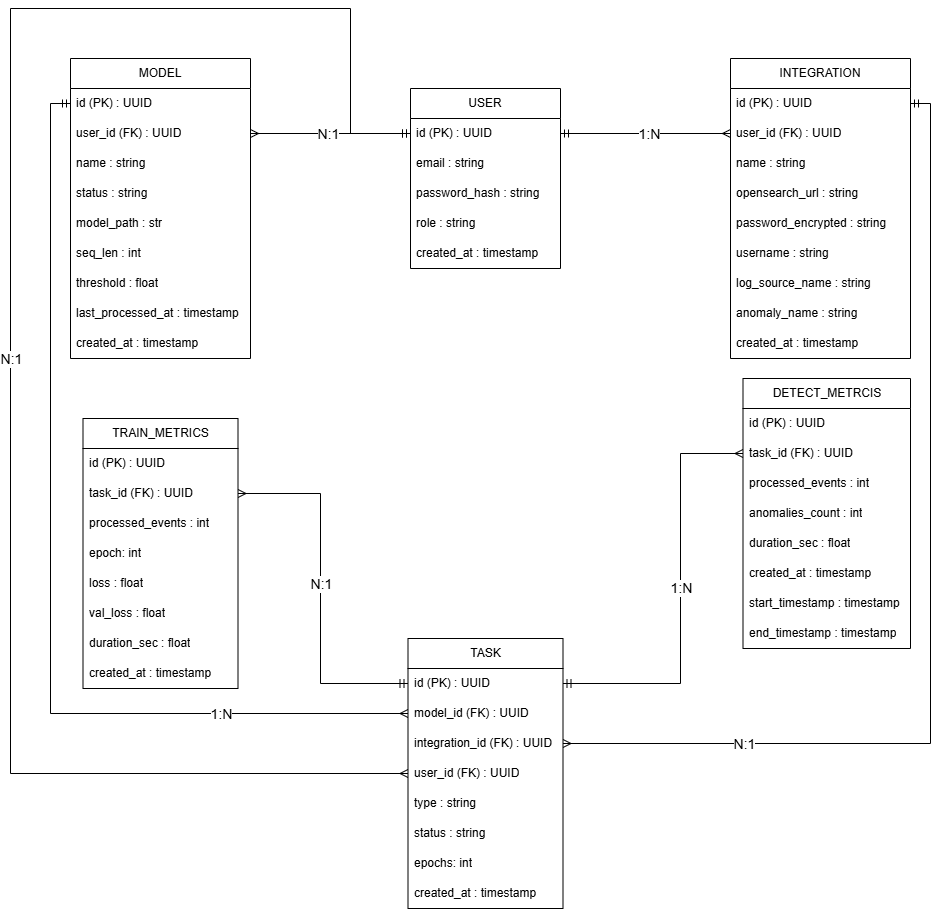
\includegraphics[scale=0.5]{inc/images/db_uml}
    \caption{UML-диаграмма базы данных программного средства}
    \label{fig:db_uml}
\end{figure}


В базе данных выделены следующие основные сущности:

\begin{itemize}
    \item \textit{User} — хранит информацию о пользователях системы, включая учётные данные и роль;
    \item \textit{Integration} — описывает подключение к источнику данных OpenSearch и содержит параметры доступа;
    \item \textit{Model} — хранит информацию о моделях НС, включая путь до весов модели в S3-хранилище, текущий статус модели, порог обнаружения аномалий;
    \item \textit{Task} — представляет задачи системы (обучение или обнаружение), выполняемые worker-компонентами;
    \item \textit{Train\_Metrics} — хранит метрики обучения моделей на различных эпохах;
    \item \textit{Detect\_Metrics} — содержит результаты выполнения задач на обнаружение аномалий в audit-логах за определенный период, включая статистику обработки и количество обнаруженных аномалий.
\end{itemize}
